%%%%%%%%%%%%%%%%%%%%%%%%%%%%%%%%%%%%%%%%%%%%%%%%%%%%%%%%%%%%%%%%%%%%%%%%%%%%%%%%%%%%%%%%%%%%%
%									Chapitre 1												%
%%%%%%%%%%%%%%%%%%%%%%%%%%%%%%%%%%%%%%%%%%%%%%%%%%%%%%%%%%%%%%%%%%%%%%%%%%%%%%%%%%%%%%%%%%%%%
\chapter{Etat de l'art}
	\citationChap{
	If I knew how I knew everything I knew, then I would only be able to know half has much, because it will all be clogged up with where I know it from. So I cannot always cite my sources, I'm sorry.
	}{David Mitchell}
	\minitoc
	\newpage

%%%%%%%%%%%%%%%%%%%%%%%%%%%%%%%%%%%%%%%%%%%%%%%%%%%%%%%%%%%%%%%%%%%%%%%%%%%%%%%%%%%%%%%%%%%%%



% Début du chapitre


\section{La perception visuelle}
\subsection{L'inspiration biologique}
\subsection{L'émergence}
\subsection{Particularités de la vision}
\subsection{Cortex visuel humain}
\subsection{Méthodes classiques informatiques}

\newpage
\section{Réseaux neuronaux}
\subsection{Cartes auto organisatrices}

	Les cartes auto-organisatrices (aussi appellées réseaux de Kohonen) regroupent un ensemble de modèles qui a commencé par une publication de Teuvo Kohonen \cite{kohonen-som82}. Ces modèles sont caractérisés par leur capacité à projeter des données de façon ordonnée sur un espace d'une dimension plus faible (typiquement une ou deux dimensions). Cette réduction dimensionnelle donne ainsi une "carte" représentative des données qu'on lui a fourni, car les propriétés de voisinages sont conservées. Une des premières utilisation de ces cartes fut la représentation des phonèmes du finnois comme présenté dans la figure \ref{fig:img:phonemes}.

	\begin{figureth}
		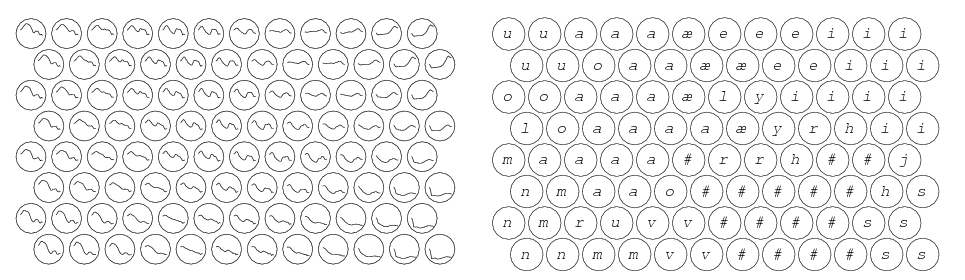
\includegraphics[width=\linewidth]{kohonen_phonemes}
		\caption[Phonème SOM]{Représentation des phonèmes du finnois par la première SOM. A gauche sont représentés les signaux sonores en haute dimension, et à droite leurs phonèmes correspondants. La réduction dimensionnelle provient de l'agencement de ces phonèmes sur la carte. Si ils sont proches entre eux dans leur espace d'entrée (signal), ils seront également proches dans la carte (la position des bulles). \textit{source : scholarpedia}}\label{fig:img:phonemes}

	\end{figureth}

	Le but premier de Kohonen était de présenter un modèle capable de représenter informatiquement l'organisation spatiale des informations dans le cortex humain \cite{kohonen-memory}. 
	
	Il s'inspira pour cela du concept neuroscientifique de colonnes corticales. Les colonnes corticales sont un groupe de neurones arrangées verticalement et qui réagissent tous au même stimulus.

\subsubsection{Evolutions et utilisation contemporaine}
	Il y a eu de nombreuses évolutions pendant les presque 40 années d'existence des SOM. En 2002, une bibliographie recensait 5384 articles scientifiques utilisant les SOM \cite{oja2003bibliography}. Ils étaient estimés à plus de 10000 en 2011 \cite{bilbiography-finuni}. Les domaines d'applications sont très variés, allant de l'image et la vidéo, par la parole et le traitement du signal, la médicine et la biologie, l'économie et la finance, de l'urbanisme et d'autres encore. Pour chacun de ces domaines il y a plusieurs types d'utilisations différentes de la SOM. Elle peut par exemple être utilisée en tant que méthode de visualisation capable de rendre humainement interprétable des données à très grande dimension et en les projetant sur des dimensions plus petites. Mais aussi pour faire des traitements sur des données, par exemple pour faire de la classification non supervisée de caractères, de chiffres ou de phonèmes, ou de la détection d'anomalies entre autres. \cite{cottrell2018self} est une revue récente évoquant les aspects les plus importants des SOM et présentant quelques applications typiques. 

	Evolutions et dérivés.

\subsection{Principes de fonctionnement}
\subsubsection{Préparation des données}

	Nous présentons dans cette section le fonctionnement de l'algorithme de la SOM que nous avons utilisé. Notre version est tout à fait classique et correspond à ce qui est communément utilisé dans la littérature.\\

	Les données présentées à la SOM doivent être numériques et sous forme de vecteurs. La taille des vecteurs peut être aussi grande que nécessaire, mais toutes les données de la bases doivent avoir la même taille de vecteur. Nous n'avons utilisé que des données normalisées, c'est à dire, dont la valeur est comprise entre 0 et 1 inclus. Par exemple pour apprendre des couleurs avec une SOM, on pourra représenter chaque couleur par un vecteur de taille 3, un élément par composante R,G et B par exemple et renormalisée pour être comprise entre 0 et 1. L'ordre de présentation des vecteur est aléatoire.

\subsubsection{Paramètres}\label{param_som}

	La forme de la SOM dépend de plusieurs paramètres. Le premier est la dimensionalité. Les SOM peuvent aller d'une dimension de un à un nombre arbitrairement grand. Cependant, en pratique elles ne dépassent que rarement deux dimensions. La raison est que la visualisation est plus aisée en deux dimensions pour toutes les applications où cela en est le but premier. C'est aussi la taille idéale pour profiter de la réduction dimensionnelle sans pour autant augmenter de façon exponentielle les coûts en calculs à taille de carte égale. Une carte de 10 neurones de côté aura 100 neurones en deux dimensions et 1000 en 3 dimensions, les coûts en calculs étant proportionnels au nombre de neurones. Nous avons ainsi utilisé exclusivement des cartes bidimensionnelles dans nos expériences. Dans notre cas, nous avons également pris en compte la contrainte matérielle qui rend les toutes les dimensions supérieures à deux difficiles à implémenter efficacement dû à des coûts en communication accrus, car les circuits imprimés sont naturellement en deux dimensions.
	
	Un second choix important est ce que nous appellons la topologie de la SOM. Par topologie, nous entendons la forme des connections entre les neurones qui composent la SOM. Les deux topologies les plus communes pour les SOM sont en grille et hexagonale. Dans la topologie en grille chaque neurone a quatre voisins, un à chaque direction cardinale. En hexagone, chaque neurone a 6 voisins, formant un pavage hexagonal avec les neurones au centre des hexagones. Ces topologies sont deux dimensionnelles, mais il est possible de les rendre toriques ou sphériques. Nous n'explorererons pas cette possibilité dans cette thèse, car cela apporte en général plus de contraintes topologiques, c'est plus difficile pour une sphère de bien couvrir les données que pour une surface plane avec des degrés de libertés au extrémités. D'autres topologies plus exotiques existent et possèdent des propriétés intéressantes \cite{bernard2018np}, cependant nous avons dû nous limiter aux topologies classiques, les différences entre les topologies des SOM n'étant pas notre objet d'étude ici.

	Le dernier type de paramètre pour la SOM sont les paramètres numériques. Il y a parmi ceux-ci : La taille de la SOM, communément notée $n$. Elle défini le nombre de neurones par côté de la SOM. Le nombre total de neurones $N$ est obtenu à partir du carré des côtés : $n^2$. Dans le cas d'une SOM non-carrée, on notera $l$ et $h$ respectivement sa largeur et sa hauteur. Il y a aussi le coefficient d'apprentissage $\epsilon$ (epsilon), défini dans $]0,1[$. Il est décroissant linéairement tout au long de l'apprentissage, On notera dans cette thèse la valeur de départ et la valeur finale, toutes les valeurs intermédiaires seront extrapolées par la droite qui coupe ces deux points en fonction de l'étape courante de l'apprentissage. Le dernier paramètre est le coefficient de voisinage $\sigma$ (sigma), défini dans $[0,1[$. Il sert à définir l'impact des neurones voisins sur les poids du neurone courant. Plus il est élevé, plus les voisins ont un impact et plus la contrainte topologique sera forte. Inversement, une valeur de 0 pour ce paramètre enlève toute contrainte topologique et fait que la SOM se comportera comme un k-means. Comme pour le coefficient d'apprentissage, il décroit linéairement pendant l'apprentissage et nous n'indiquerons que les valeurs de départ et de fin.

\subsubsection{Apprentissage}

	Au début de l'apprentissage, tous les poids des neurones sont initialisés aléatoirement entre 0 et 1. L'apprentissage dure un certain nombre d'époques définies avant lancement. Une époque contient exactement le nombre d'itérations requises pour que chaque élément de la base d'apprentissage soit utilisé exactement une seule fois par époque. Lors d'une itération, on sélectionne aléatoirement un vecteur d'apprentissage parmi la base d'apprentissage, qui n'a pas déjà été utilisé lors de cette époque. 

	Une itération se déroule en deux étapes : 
	\begin{itemize}
		\item La phase de recherche, qui consiste à trouver la \textit{Best Matching Unit} (BMU) parmi tous les neurones. Elle correspond au neurone qui a la plus petite distance $L^2$ (distance euclidienne), entre ses poids et le vecteur d'apprentissage.
		\item La phase d'adaptation, qui modifie les poids des neurones selon l'équation suivante :
		\begin{equation}\label{eq:SOM}
			w_i(t+1) = w_i(t)+\epsilon(t)\cdot\Theta(\sigma(t),d_{i,bmu})\cdot(v-w_i(t))
		\end{equation} avec $i$ le neurone courant, $w_i$ les poids de ce neurone, $t$ l'itération courante, $\epsilon$ et $\sigma$ des paramètres de la SOM définis dans la section \ref{param_som}. $d_{i, bmu}$ est la distance $L^1$ (distance de manhattan) normalisée entre le neurone $i$ et la BMU. $\Theta$ est une fonction gaussienne centrée normalisée d'écart type $\sigma$. $v$ est la vecteur d'apprentissage.
	\end{itemize}

	On répète ces deux étapes jusqu'à ce que l'on finisse la dernière époque, est l'apprentissage sera terminé.

\subsubsection{Reconstruction}
	
	On appelle reconstruction le fait de remplacer un ensemble de vecteurs, de longueur similaire à ceux sur laquelle la SOM a été apprise, par les poids des neurones les plus proches.

	Cette reconstruction est par exemple utilisée pour de la compression de données, car à la place de mémoriser un ensemble de vecteurs, il n'y a besoin que de mémoriser les poids de la SOM et l'indice de chaque neurone le plus proche de chaque vecteur de l'ensemble. Cette compression est avec perte, du fait que les poids des neurones sont en général pas exactement les mêmes que les vecteurs présentés, même lorsque ceux-ci faisaient partie de la base d'apprentissage.

	\subsection{Gaz Neuronaux en Expansion}

	Bien que nos travaux se soient focalisés sur les cartes auto-organisatrices, notre approche se veut généraliste et transposable à d'autres modèles de quantification vectorielle avec topologie. Nous avons souhaité valider expérimentalement cette transposition en utilisant les Gaz neuronaux en expansion. C'est un autre modèle similaire aux SOM mais avec une approche tout à fait différente sur la topologie, qui devient dynamique et non pas fixe. 

	\subsubsection{Développements}

	Une évolution majeure inspirée par les carte auto-organisatrices a été le développement des différents types de gaz neuronaux (Neural Gases, NG), qui a commencé avec \cite{martinetz1991neural}, en tant qu'alternative aux k-means car ils ne disposent pas de topologie non plus. Puis ce sont les Gaz Neuronaux en Expansion (Growing Neural Gases, GNG) \cite{fritzke1995growing} qui ont sensiblement amélioré l'approche en ajoutant un mécanisme de croissance qui ajoute des neurones lors de l'apprentissage et une topologie avec des connexions qui se créent et qui disparaissent entre les neurones.

	De nos jours, plusieurs variantes des GNG existent qui améliorent certains aspects de cet algorithme. Notablement, Growing when required \cite{marsland2002self} adapte la croissance du nombre de neurones en fonction de ce que le réseau à déjà appris, produisant une forte neurogénèse au début de l'apprentissage et une stabilisation une fois que les données ont été suffisament apprises. Une autre variante sont les Icremental growing neural gases \cite{prudent2005incremental}. Ils permettent d'apprendre de nouvelles données sans oublier les anciennes en combinant plasticité et stabilité.

	Pour la suite, nous avons décidé d'utiliser uniquement l'algorithme des Gaz neuronaux en expansion. C'est le plus utilisé, et les avantages qu'apportent les variants ne sont pas nécessaires dans notre cas.

	\subsubsection{Fonctionnement}

	Nous ne présenterons le fonctionnement que des gaz neuronaux en expansion. L'algorithme ne se réduisant pas aisément en quelques formules, nous prendrons une approche itérative, similaire à celle que l'on peut trouver dans l'article original, pour expliquer les différents mécanismes à l'oeuvre.\\

	Une itération se décompose en 9 étapes :
	\begin{enumerate}
		\item Choisir au hasard un élément de la base d'apprentissage parmi ceux qui n'ont pas déjà été tirés lors de cette époque.
		\item Trouver les deux neurones les plus proches : $s_1$ et $s_2$.
		\item Incrémenter l'âge des synapses de tous les voisins topologiques directs de $s_1$.
		\item Ajouter la distance euclidienne au carré entre le vecteur d'apprentissage et $s_1$ à la variable d'erreur de $s_1$.
		\item Mettre à jour les poids de $s_1$ et de tous ces voisins topologiques directs $s_n$. Les formules sont :
		\begin{equation}
			w_{s_1}(t+1) = w_{s_1}(t) + \epsilon_{\textit{bmu}} \times (v - w_{s_1}(t))
		\end{equation}
		\begin{equation}
			w_{s_n}(t+1) = w_{s_n}(t) + \epsilon_{n} \times (v - w_{s_n}(t))
		\end{equation}
		\item Si $s_1$ et $s_2$ sont voisins topologiques directs, mettre à jour l'âge de la synapse à 0. Sinon créer une synapse.
		\item Enlever toutes les synapses avec un âge supérieur à $a_{\textit{max}}$. Si des neurones se retrouvent sans synapses, les enlever aussi.
		\item Si l'itération courante est un multiple de $\lambda$, insérer un nouveau neurone comme suit :
		\begin{itemize}
			\item Trouver le neurone avec l'erreur la plus élevée $q$.
			\item Créer un nouveau neurone $r$ à distance égale de $q$ et de son voisin direct avec l'erreur la plus élevée $f$.
			\begin{equation}
				w_r(t+1) = \frac{w_q(t) + w_f(t)}{2}  
			\end{equation}
			\item Ajouter des synapses d'âge 0 entre $r$ et $q$ ainsi qu'entre $r$ et $f$. Enlever la synapse entre $q$ et $f$.
			\item Réduire l'erreur de $q$ et $f$ en la multipliant par une constante $\alpha$. Initialiser l'erreur de $r$ avec la nouvelle valeur de l'erreur de $q$.
		\end{itemize}
		\item Réduire toutes les variables d'erreur en les multipliant par une constante $d$.
	\end{enumerate}\text{\\}

	L'apprentissage s'arrête au bout d'un certain nombre prédéfini d'époques, comme pour la SOM. L'effet de chaque paramètre peut être compris aisément par le contexte dans lequel il est utilisé, ainsi nous n'irons pas de le détail de chacun d'entre eux. Le paramètre $\lambda$, ajustant la vitesse de création de nouveaux neurones, sera fixé de telle sorte qu'à la fin de l'apprentissage il y ait le même nombre de neurones dans le GNG que dans la SOM à laquelle on souhaite se comparer. La reconstruction se passe de la même façon que pour la SOM. Les valeurs que l'on aura utilisées pour nos paramètres sera précisée dans la section expérimentale correspondante.

	\subsection{DNF}

	

	Following the seminal work of \cite{Fix:dnf:2011}, we choose to couple our autonomous novelty detection tool to a robust bio-inspired tracking technique based on Dynamic Neural Fields (DNF). DNF are populations of partial differential equations first mathematically analyzed by \cite{amari:dnf:1977} in a continuous framework. We use a discrete DNF built from populations of excitatory and inhibitory neurons that interact continuously, with a on-center off-surround approach modeled as a synaptic kernel computed as a difference of gaussians applied to the distance between neurons in the neural map. These DNF have been successfully applied to sequential visual exploration of an environment \cite{Fix:dnf:2011} or in \cite{rougier:attention:2005}, with great robustness properties that can even improve with some adaptation like the use of simple spiking neurons \cite{vazquez:dnf:2011}. 

	\subsubsection{Fonctionnement}

	Continuous Neural Fields Theory (CNFT) has lead to the development of two dimensional Dynamic Neural Fields (DNF) \cite{Taylor2D}. Neural fields are models that represent the evolution of a population of neurons. In our case, we use a two dimensional DNF. The number of neurons is dependent and equal to the size of the input map, because neurons are connected in a retinotopic way to afferent inputs, and are connected in an all-to-all connection scheme between them. All neurons also have a real value attached to them that we call potential. This potential $u(x,t)$, with $x$ being the neuron position in the field and $t$ the time of the simulation, is ruled by the following differential equation :

$$\tau \frac{\partial u(x, t)}{\partial t} = -u(x,t)+\int u(x',t)\omega(||x-x'||)\delta y + \text{Input}(x,t)$$

With :
\begin{itemize}
    \item $\tau$ is the time constant.
    \item $-u(x,t)$ is the decay term. It is meant to suppress already activated neurons when there is no input or lateral excitation.
    \item $\omega(||x-x'||)$ is the lateral interaction. It represents the effect of the other neurons onto this neuron's potential. We are using a difference of gaussian with the excitatory gaussian part being narrow with high intensity and the inhibitory one being wide with low intensity. This leads to close neurons having an excitatory effect onto each other and far away neurons inhibiting themselves.
    \item $Input(x,t)$ is the current value of the afferent input extracted from the input map for this neuron.
\end{itemize}

For the sake of simplicity and computability, we implement a spatially and temporaly discretized version of the previous formula. It is obtained by handling potentials of a discrete set of neurons (neural map instead of neural manifold) and by using a simple Euler method to estimate the state of $u(x,t+\Delta t)$ knowing $u(x,t)$:

$$u(x, t+\Delta t) = u(x, t) +\frac{\Delta t\left(-u(x, t)+\sum u(x', t)\omega(||x-x'||) + \text{Input}(x, t+\Delta t)\right)}{\tau}$$

$\Delta t$ is the time step between two estimations, it can be the same for all neurons (synchronous) or different each time (asynchronous). It should be noted that in the original DNF formula, there are more parameters such as resting potential but since we do not use them here, we did not mention them.

It is often difficult to understand how a DNF will behave just from the formula. We have set it up with optimized parameters in order to have a winner-takes-all behaviour where the most prominent and spatially coherent features in the input map create a local bubble of activation in the neural map and suppress the ability of other such bubbles to appear elsewhere in the map. 

\newpage
\section{Matériel Neuromorphique}
\subsection{Processeurs}
\subsection{Caméra évènementielles}

\bibliographystyle{francaissc}
\bibliography{Chapitre1/Biblio}